\documentclass[tikz,border=2pt]{standalone}
\usepackage{amsmath}
\usetikzlibrary{arrows.meta}
\begin{document}
% Timing of a static Bayesian game: Nature draws theta from the common prior p; player i sees only
% theta_i and plays a_i = s_i(theta_i); payoffs v_i(a; theta) depend on all actions and all types.
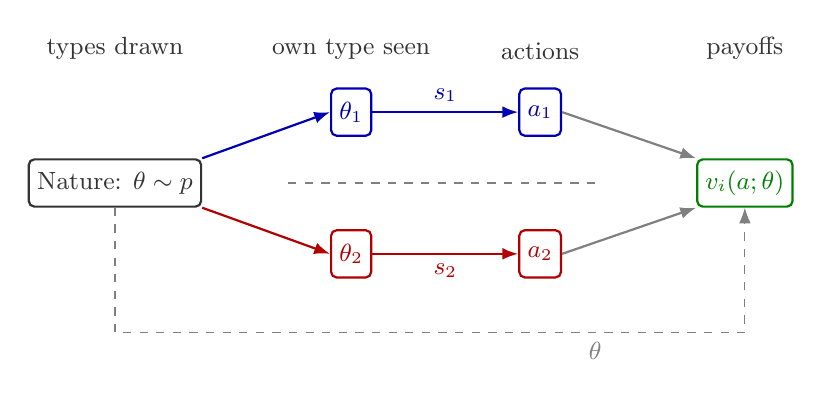
\begin{tikzpicture}[font=\small, >={Latex[length=2mm]},
    box/.style={draw, thick, rounded corners=2pt, inner sep=3pt, minimum height=6mm}]
  \node[box, gray!40!black] (N) at (0,0) {Nature: $\theta\sim p$};
  \node[box, blue!70!black] (t1) at (3.0,0.9) {$\theta_1$};
  \node[box, red!70!black] (t2) at (3.0,-0.9) {$\theta_2$};
  \node[box, blue!70!black] (a1) at (5.4,0.9) {$a_1$};
  \node[box, red!70!black] (a2) at (5.4,-0.9) {$a_2$};
  \node[box, green!50!black] (v) at (8.0,0) {$v_i(a;\theta)$};
  \draw[->, thick, blue!70!black] (N.north east) -- (t1.west);
  \draw[->, thick, red!70!black] (N.south east) -- (t2.west);
  \draw[->, thick, blue!70!black] (t1) -- node[above] {$s_1$} (a1);
  \draw[->, thick, red!70!black] (t2) -- node[below] {$s_2$} (a2);
  \draw[->, thick, gray] (a1.east) -- (v.north west);
  \draw[->, thick, gray] (a2.east) -- (v.south west);
  % payoffs also depend on the full type profile
  \draw[->, thin, dashed, gray] (N.south) |- (4.2,-1.9) -| node[pos=0.25, below] {$\theta$} (v.south);
  % separation of private information
  \draw[thin, dashed, gray] (2.2,0) -- (6.2,0);
  % stage labels
  \node[gray!40!black, anchor=south] at (0,1.45) {types drawn};
  \node[gray!40!black, anchor=south] at (3.0,1.45) {own type seen};
  \node[gray!40!black, anchor=south] at (5.4,1.45) {actions};
  \node[gray!40!black, anchor=south] at (8.0,1.45) {payoffs};
\end{tikzpicture}
\end{document}
